\documentclass[border=7pt]{standalone}
\usepackage{amsmath,amssymb,bm,mathtools}
\usepackage[fontset=none]{ctex}
\setCJKmainfont{Songti SC}\setCJKsansfont{PingFang SC}
\usepackage{tikz}\usetikzlibrary{arrows.meta,calc,patterns,angles,quotes,decorations.markings,decorations.pathmorphing}
\newcommand{\dd}{\mathop{}\!\mathrm d}
\definecolor{blue}{HTML}{235789}\definecolor{red}{HTML}{BC4B41}
\tikzset{axis/.style={->,>=Stealth,line width=.55pt},world/.style={line width=.9pt},flow/.style={->,>=Stealth,line width=.85pt},ray/.style={->,>=Stealth,line width=.85pt},guide/.style={dashed,line width=.4pt},aux/.style={dashed,line width=.4pt},dim/.style={<->,>=Stealth,line width=.5pt},every node/.style={font=\normalsize},force/.style={->,>=Stealth,very thick},gas/.style={fill=blue!7}}
\begin{document}
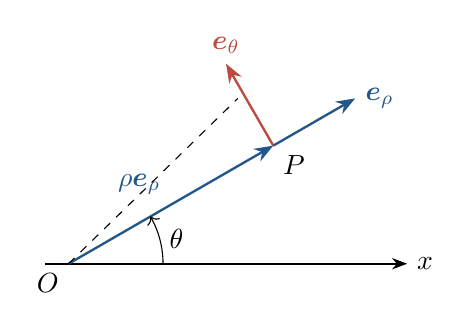
\begin{tikzpicture}
\coordinate(O)at(0,0);\coordinate(P)at(2.6,1.5);
\draw[axis](-.3,0)--(4.3,0)node[right]{$x$};
\draw[flow,blue](O)--(P)node[midway,above left]{$\rho\bm e_\rho$};
\draw[guide](O)--(2.15,2.1);
\draw[flow,red](P)--(2,2.54)node[above]{$\bm e_\theta$};
\draw[flow,blue](P)--(3.64,2.1)node[right]{$\bm e_\rho$};
\draw[->](1.2,0)arc(0:30:1.2)node[midway,right]{$\theta$};
\node[below left]at(O){$O$};\node[below right]at(P){$P$};
\end{tikzpicture}
\end{document}
